%%%%%%%%%%%%
%
% $Autor: Wings $
% $Datum: 2019-03-05 08:03:15Z $
% $Pfad: ArduinoIDEConfHypatia $
% $Version: 4250 $
% !TeX spellcheck = en_GB/de_DE
% !TeX encoding = utf8
% !TeX root = filename 
% !TeX TXS-program:bibliography = txs:///biber
%
%%%%%%%%%%%%

%source: https://randomnerdtutorials.com/installing-esp32-arduino-ide-2-0/

\chapter{Hypatia's Setup for the Arduino IDE}

\section{Introduction}

In this chapter, we will explore how to connect the board Hypatia to your computer or laptop and configure essential settings to get started. We will walk through the process of installing the necessary tools and ensuring the board is correctly set up in the Arduino IDE. Finally, we will demonstrate a simple example sketch to verify that the board is working as expected and ready for further development.


There are set of examples which are build in Arduino IDE for the testing purpose, for checking all the configuration and setting up the board we can open one of the basic example \FILE{blink.ino} first.

%%%%%%%%%%%%%%%%%%%%%%%%%%%%%%%%%%%%%%%%%%%%%%%%%%%%%%%%%%%%%%%%%%%%%%

\section{Configuration for the Arduino Nano 33 BLE Sense}

%%%%%%%%%%%%%%%%%%%%%%%%%%%%%%%%%%%%%%%%%%%%%%%%%%%%%%%%%%%%%%%%%%%%%%


To program the \textbf{Arduino Nano 33 BLE Sense} in an offline environment, follow these steps:

\begin{enumerate}
    \subsection{Installation of the driver}
    \item \textbf{Installation of the driver:} Begin by installing the latest version of the Arduino IDE on your computer. Refer to Section \ref{sec:Installation of the Arduino IDE} for more details.
    \item \textbf{Installation of the packages:} Once the IDE installation is complete, open the \menu{Arduino IDE} and navigate to the menu  \menu{Tools}.
    \item Select \menu{Tools > Board > Boards Manager\ldots}.
    \item In the window \menu{Boards Manager}, use the search bar to locate the \textbf{esp32} by typing its name as shown in Figure \ref{fig:ArduinoBoardHypatiaInstallation}		.

\begin{center}
    \begin{tikzpicture}
        \node (G) at (0,0) {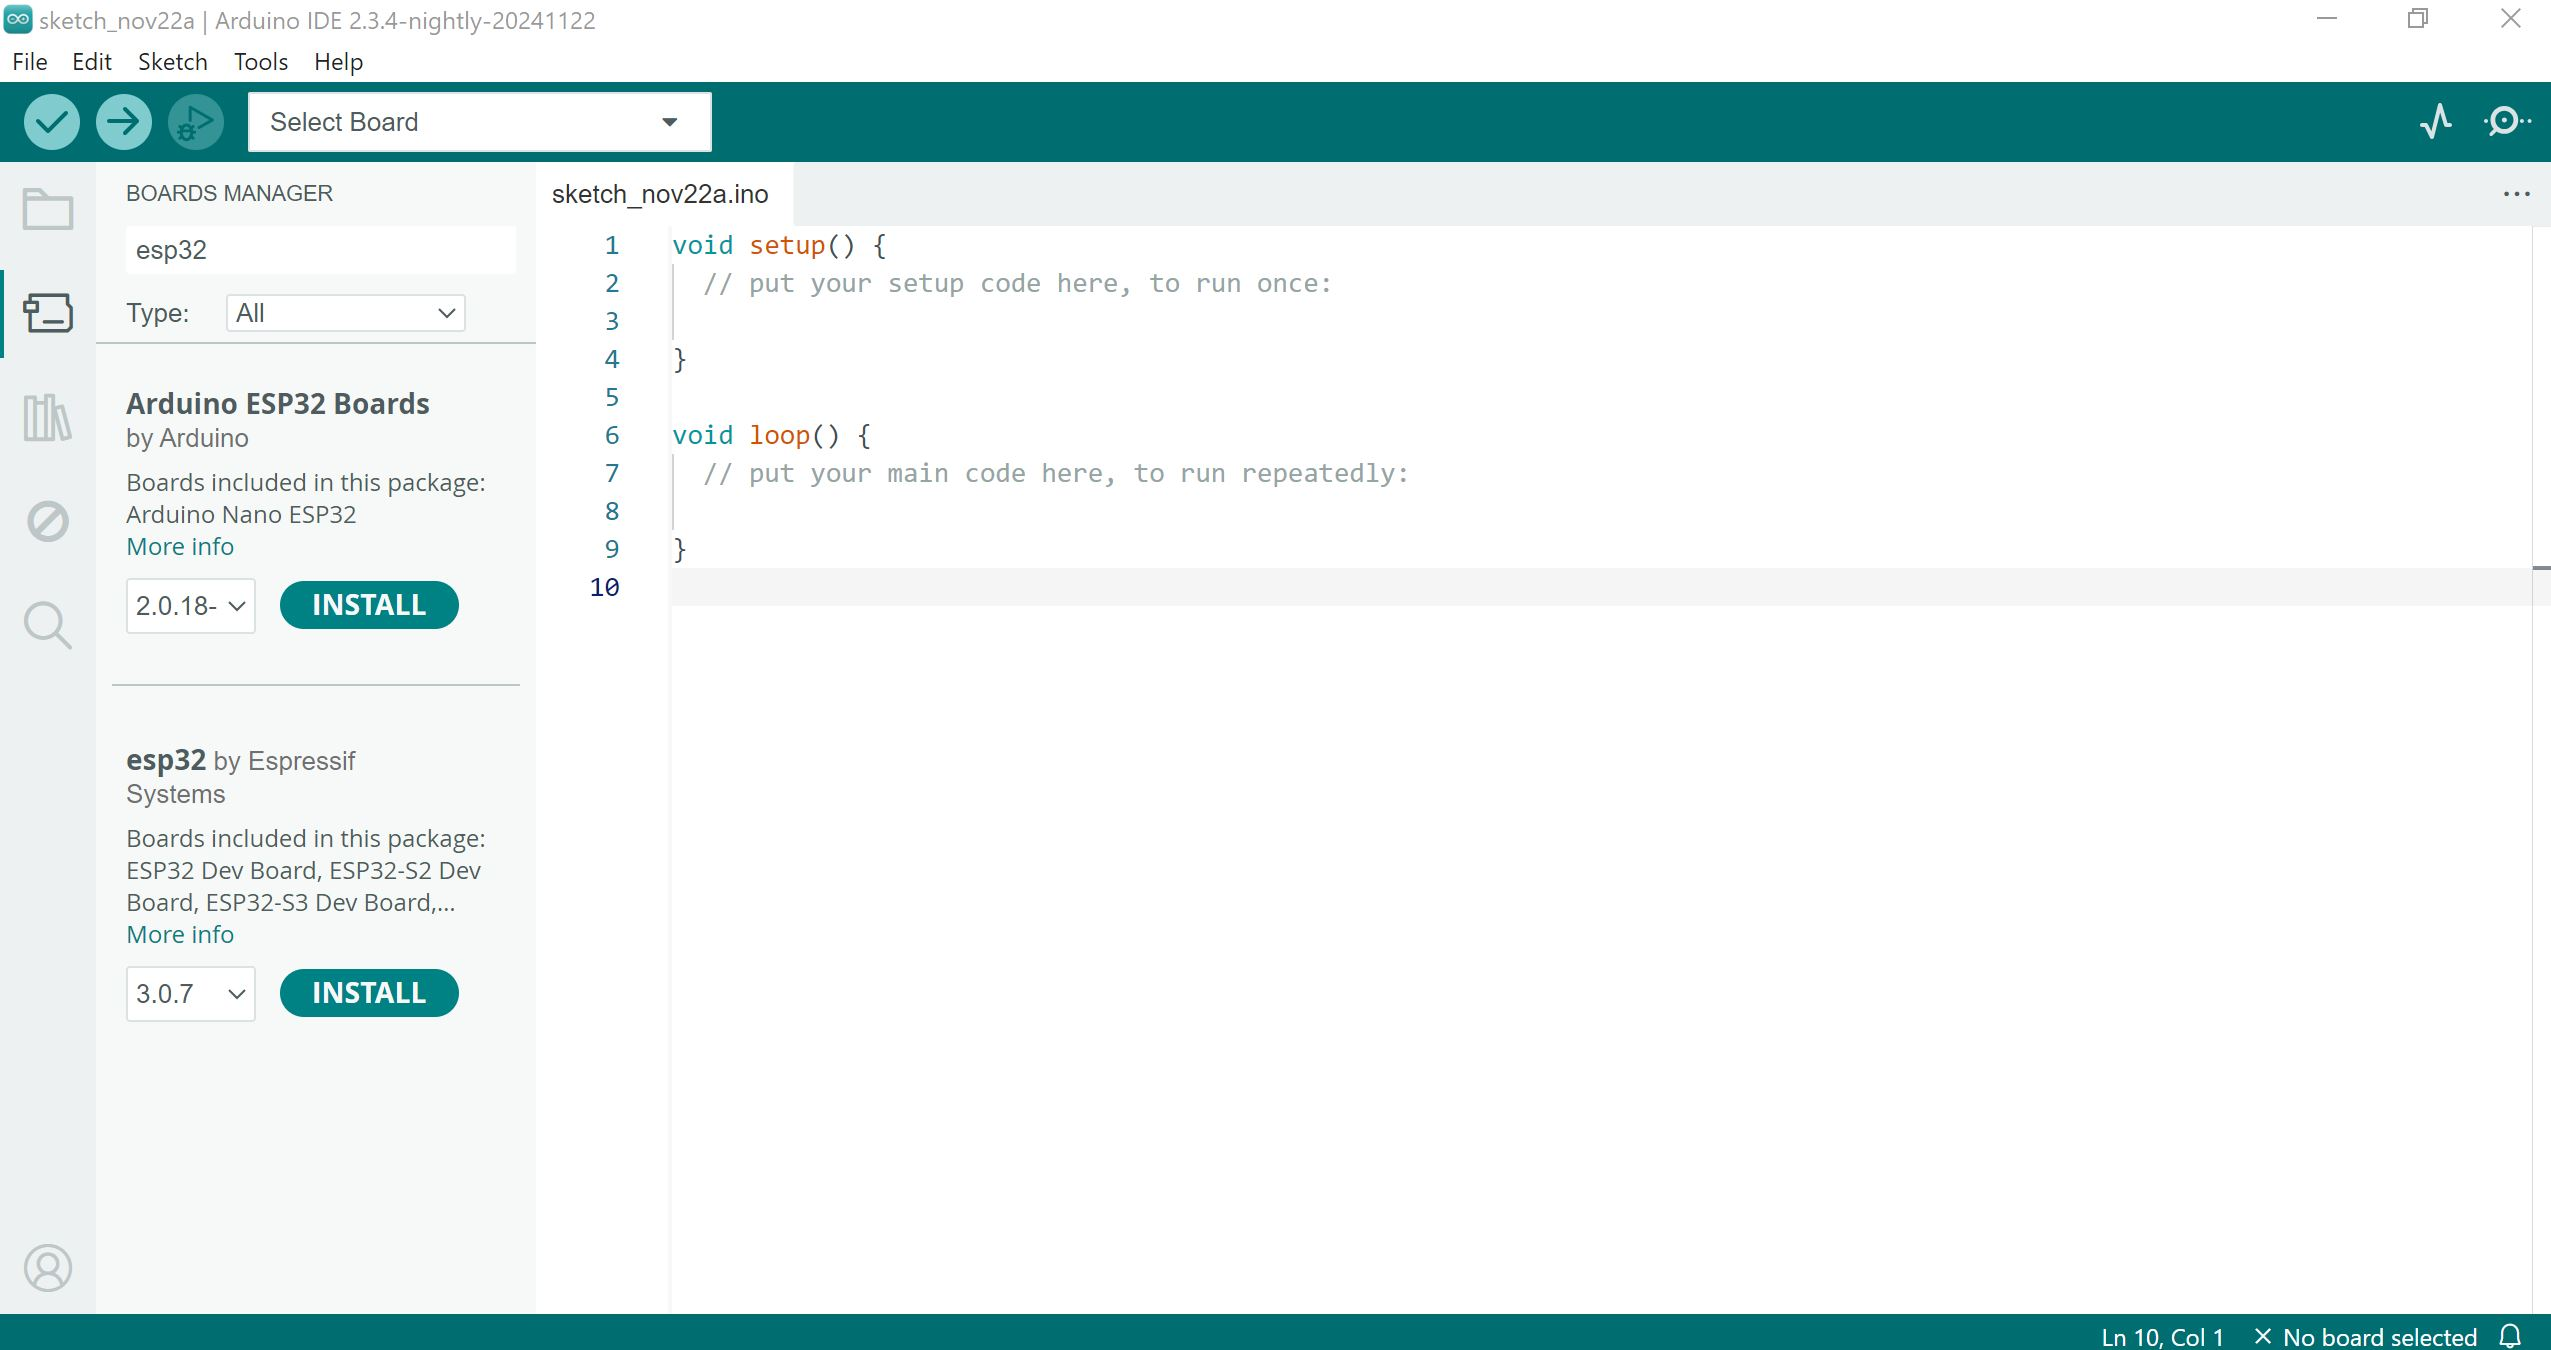
\includegraphics[width=11cm]{../../../Images/Syde/ESP32Installation}};
        
        \draw[red,domain=0:360,line width=1.4pt] plot ({-4.1+1.5*cos(\x)},{-0.9+0.75*sin(\x)});
        
        
    \end{tikzpicture}
    \captionof{figure}{Installation of the drivers for ESP32 boards}\label{fig:ArduinoBoardHypatiaInstallation}
\end{center}	

    \item Click \menu{eps32} in the search bar \menu{Select Board}. Then a window is opened.
    
    \item In the window \menu{Boards Manager}, use the search bar to locate the \textbf{Wroom} by typing its name as shown in Figure \ref{fig:ArduinoBoardHypatiaInstallation2}
    
\begin{center}
    \begin{tikzpicture}
        \node (G) at (0,0) {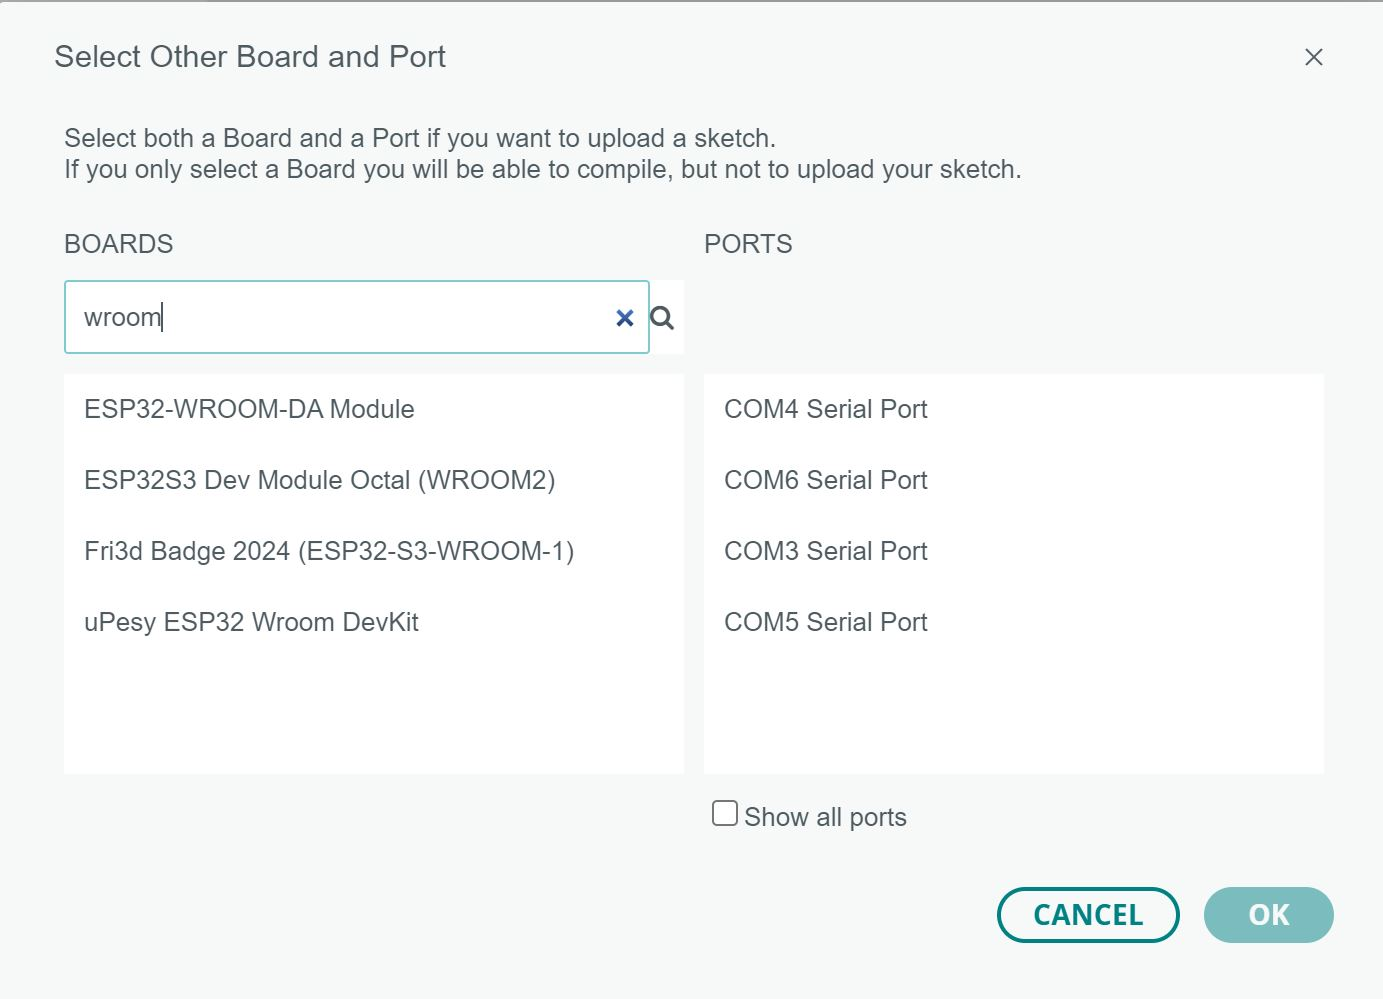
\includegraphics[width=8cm]{../../../Images/Syde/ESP32Wroom1}};
        
        \draw[red,domain=0:360,line width=1.4pt] plot ({-3.3+1*cos(\x)},{1
            +0.3*sin(\x)});
    \end{tikzpicture}
    \captionof{figure}{Search the bords ESP32-S3-WROOM-1}\label{fig:ArduinoBoardHypatiaInstallation2}
     \end{center}	
    		.
    \item From the search results, select \menu{Fri3d Badge 2024 (ESP32-S3-WROOM-1)} and click \menu{OK} to install the required package.

    \begin{center}
      \begin{tikzpicture}
        \node (G) at (0,0) {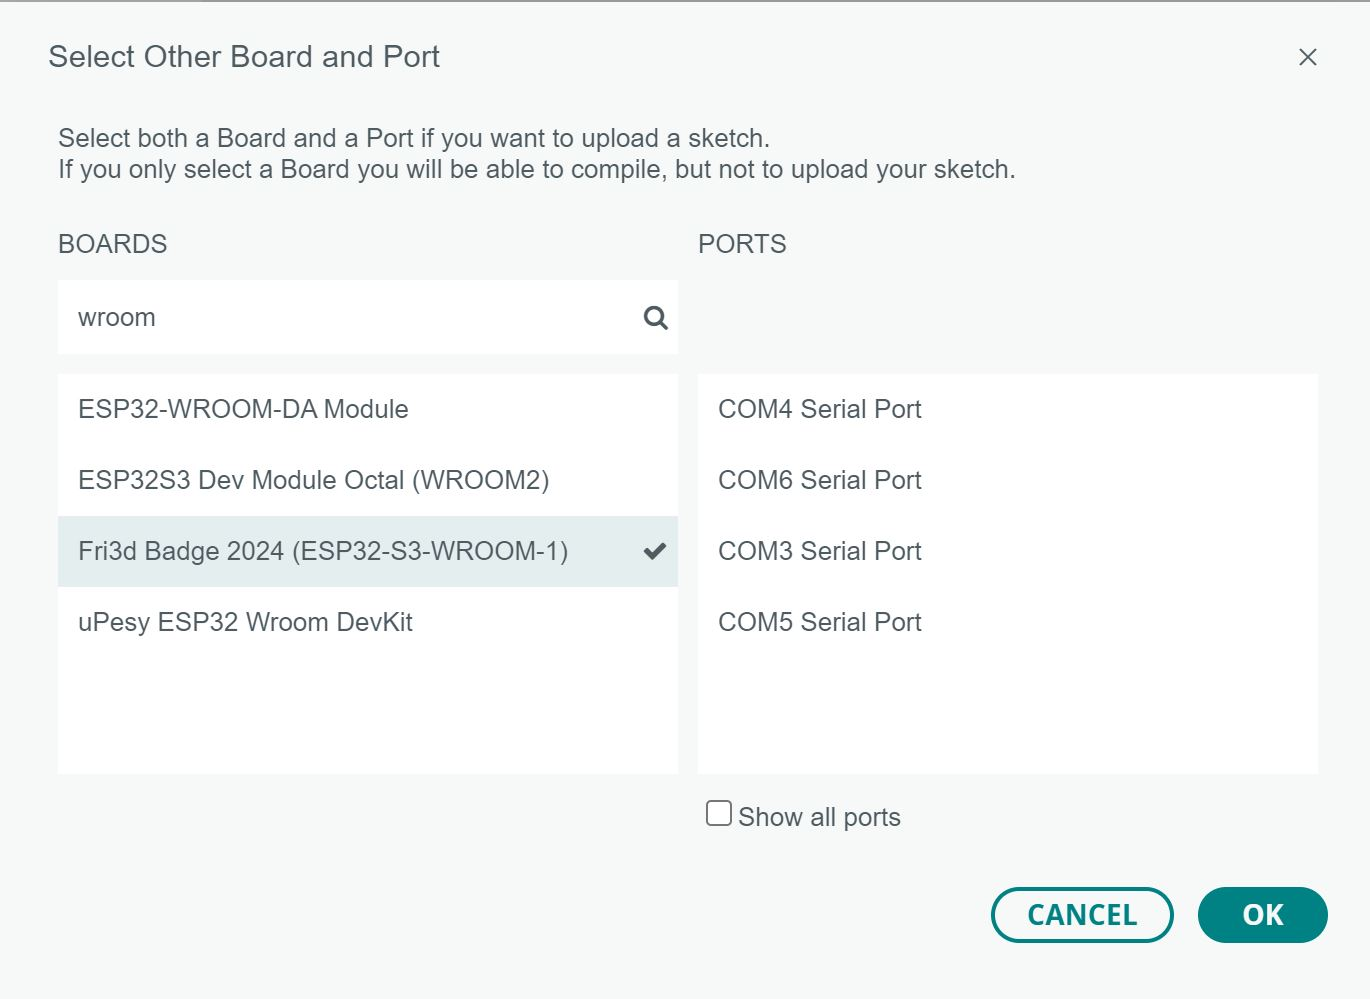
\includegraphics[width=8cm]{../../../Images/Syde/ESP32Wroom12}};
        
        \draw[red,domain=0:360,line width=1.4pt] plot ({-1.7+2*cos(\x)},{-0.3
            +0.3*sin(\x)});
      \end{tikzpicture}
      \captionof{figure}{Search the bords ESP32 Wroom-1}\label{fig:ArduinoBoardHypatiaInstallation3}
    \end{center}	
   
\end{enumerate}

The package Fri3d Badge 2024 (ESP32-S3-WROOM-1) includes support for several boards with ESP32, including Hypatia. The selected board is mentioned in the state line as shown in figure~\ref{fig:ArduinoBoardHypatiaInstallationState}.

\begin{center}
  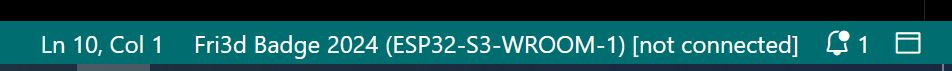
\includegraphics[width=8cm]{../../../Images/Syde/InstallationState.JPG};
        
  \captionof{figure}{Search the bords ESP32 Wroom-1}\label{fig:ArduinoBoardHypatiaInstallationState}
\end{center}	

\section{Configuration}

The Arduino IDE must be configured before using the board.

\begin{enumerate}
    \item Choose the the partition scheme: \menu{Tools > Partition Scheme > 16M Flash (3MB APP/9.9MB FATFS)}
    \item Choose the upload mode: \menu{Tools > Upload Mode > USB-OTG CDC (TinyUSB)}
    \item Choose the USB Mode: \menu{Tools > USB Mode > USB-OTG (TinyUSB)}
\end{enumerate}



\section{Connecting the Board}

After completing the installation, connect Hypatia to your computer using a USB-A to USB-C. Then the correct port must be choose: \menu{Tools > Port}. The port ``COM7'' is correct serial port in this example, see figure~\ref{fig:ArduinoBoardHypatiaConnectingState} and figure~\ref{fig:PortHypatia}.

\begin{center}
    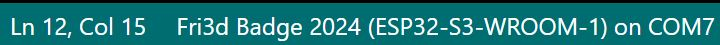
\includegraphics[width=8cm]{../../../Images/Syde/ConnectingState};
    
    \captionof{figure}{Hypatia is connected via the serial port ``COM7''}\label{fig:ArduinoBoardHypatiaConnectingState}
\end{center}	

\begin{center}
    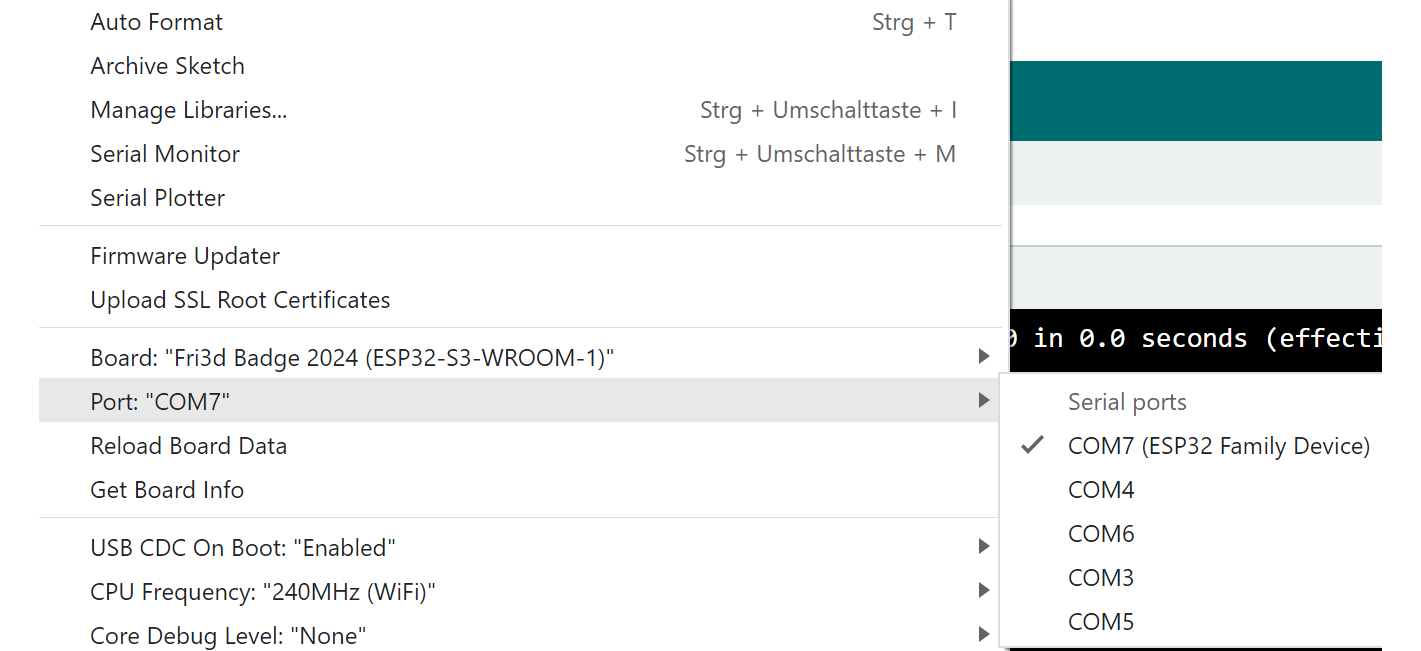
\includegraphics[width=8cm]{../../../Images/Syde/PortHypatia};
    
    \captionof{figure}{Hypatia is connected via the serial port ``COM7''}\label{fig:PortHypatia}
\end{center}	
 

%%%%%%%%%%%%%%%%%%%%%%%%%%%%%%%%%%%%%%%%%%

\section{Testing the Installation}

%%%%%%%%%%%%%%%%%%%%%%%%%%%%%%%%%%%%%%%%%%

\subsection{Loading the sketch \FILE{TestRGB.ino}}

To test the installation for Hypatia, we'll upload a simple code that blinks the onboard RGB-LED of type WS2812B. It uses the GPIO Pin 21.

\medskip

Copy the following code to your Arduino IDE:

{
    \captionof{code}{Simple sketch to control the builtin RGB-LED}\label{Syde:BuiltinRGB}
    \lstinputlisting{}{../../../Code/Syde/Test/TestRGB/TestRGB.ino}
}

The sketch uses the library \PYTHON{Adafruit NeoPixel} version 1.12.3, which has to be installed. For installation, open \menu{Tools > Manage libraries\ldots}. In the window, as shown in figure~\ref{fig:LibAdaFruitNeoPixel}, write in the search bar ``Adafruit NeoPixel'' and install the library \PYTHON{Adafruit NeoPixel} version 1.12.3.

\begin{center}
    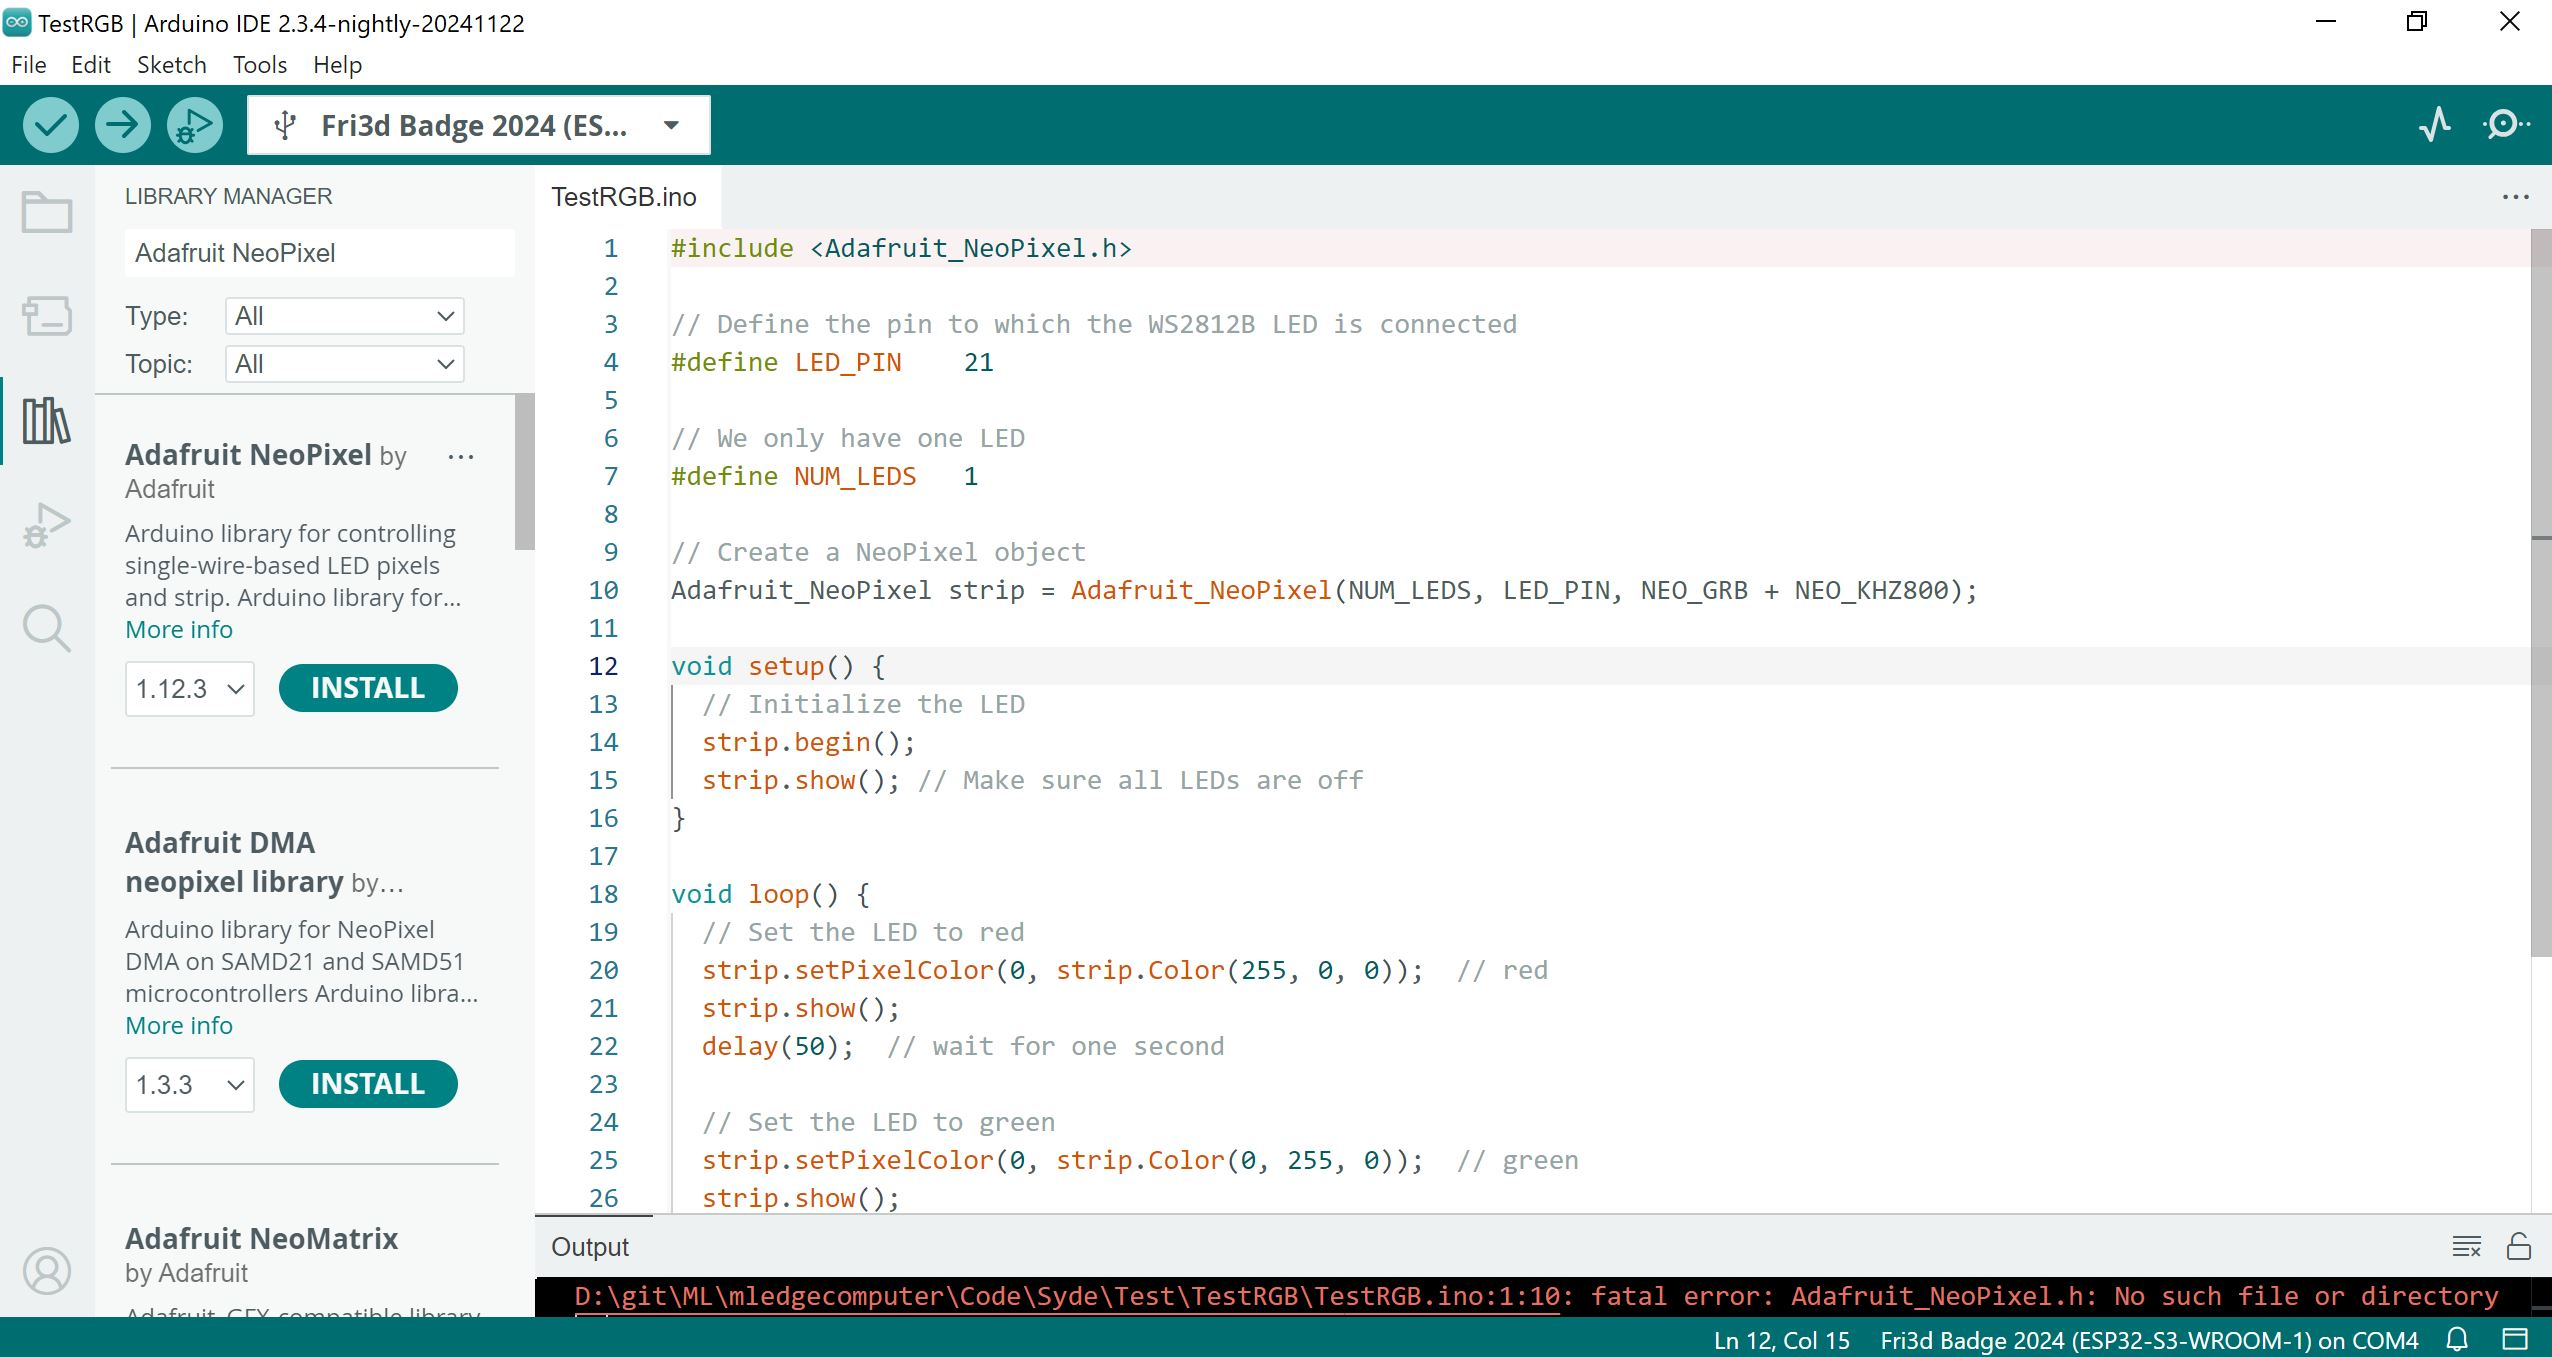
\includegraphics[width=8cm]{../../Images/Syde/LibAdaFruitNeoPixel};
    
    \captionof{figure}{Installation the library \PYTHON{Adafruit NeoPixel} version 1.12.3.}\label{fig:ArduinoBoardHypatiaConnectingState}
\end{center}	

Now, we can open the sketch \FILE{TestRGB.ino}.

Before downloading, the board must be in the mode ``download''.

\bigskip

\begin{itemize}
    \item Press the button ``Boot'' and hold.
    \item Press the button ``Reset'' once.
    \item Release the button ``Boot''.
\end{itemize}

Now, we can download the sketch. After the download, the output tells that the board must be reseted as shown in figure~\ref{fig:Donwloaded}

\begin{center}
    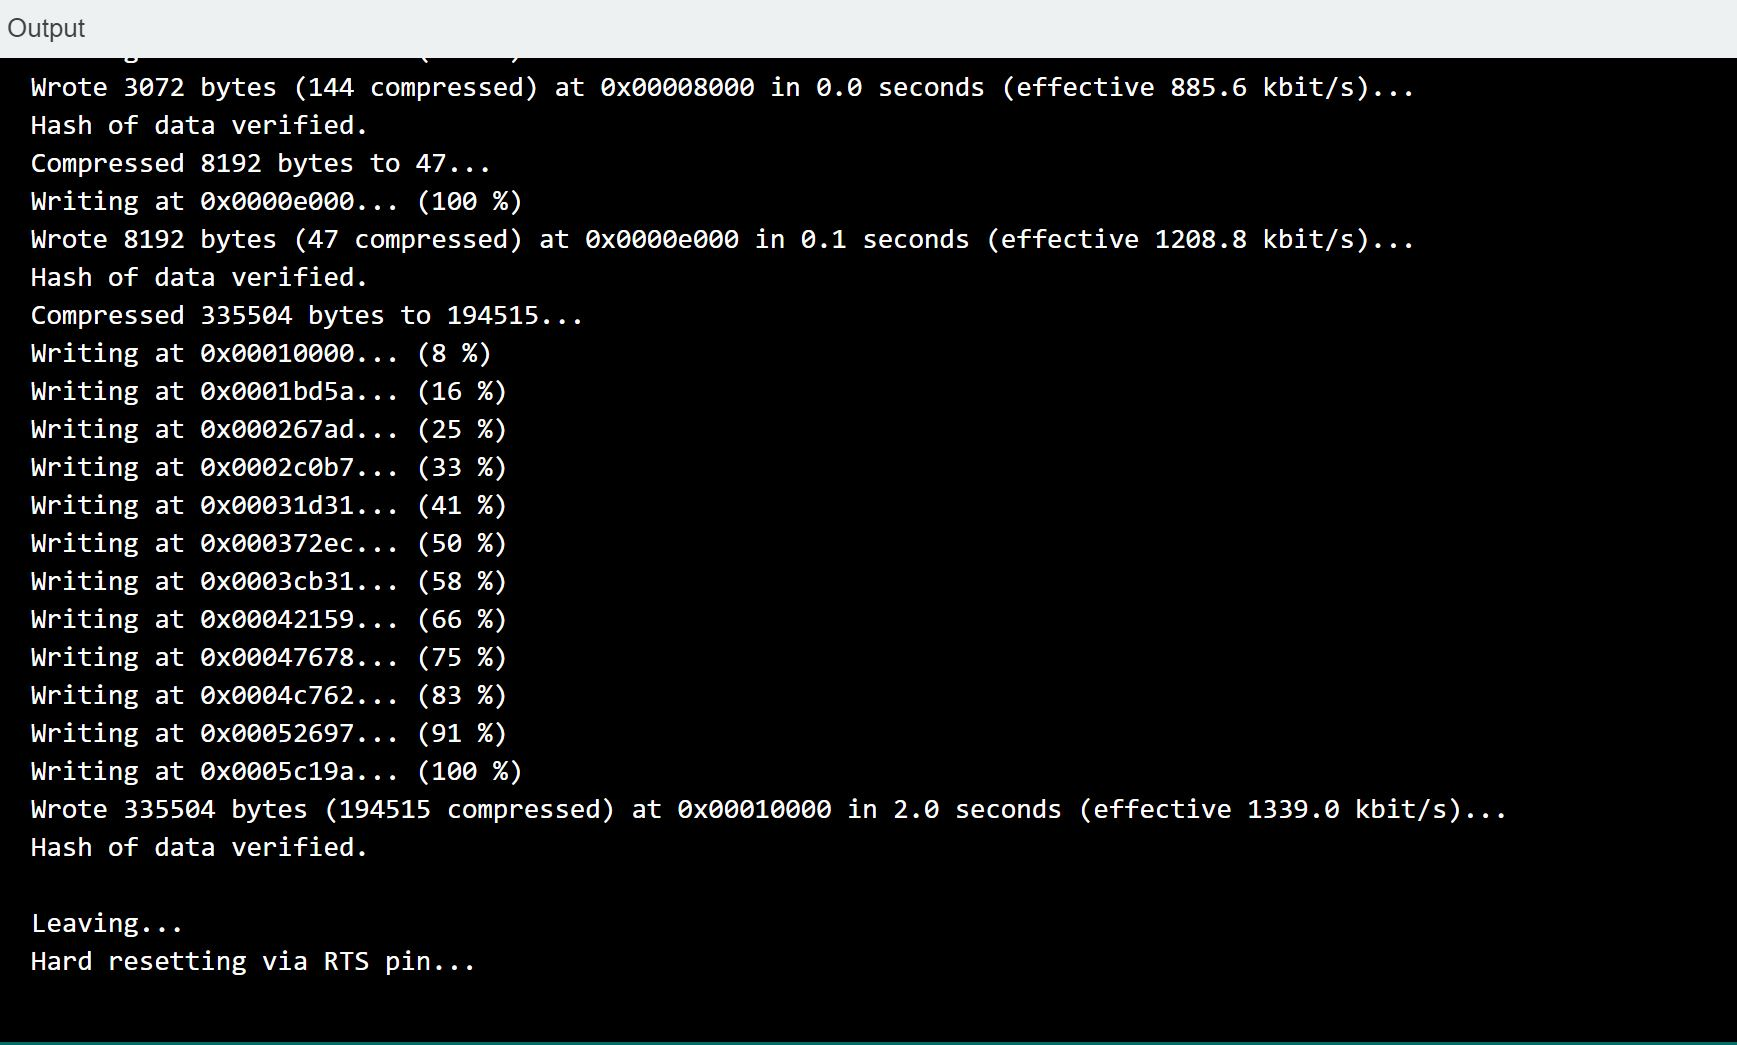
\includegraphics[width=11cm]{../../Images/Syde/Donwloaded};
    
    \captionof{figure}{Output after the download of the sketch \FILE{TestRGB.ino}}\label{fig:Donwloaded}
\end{center}	

To start the sketch, push the button ``Reset'' and the RGB LED blinks. The figure shows one moment of the situation.

\begin{center}
    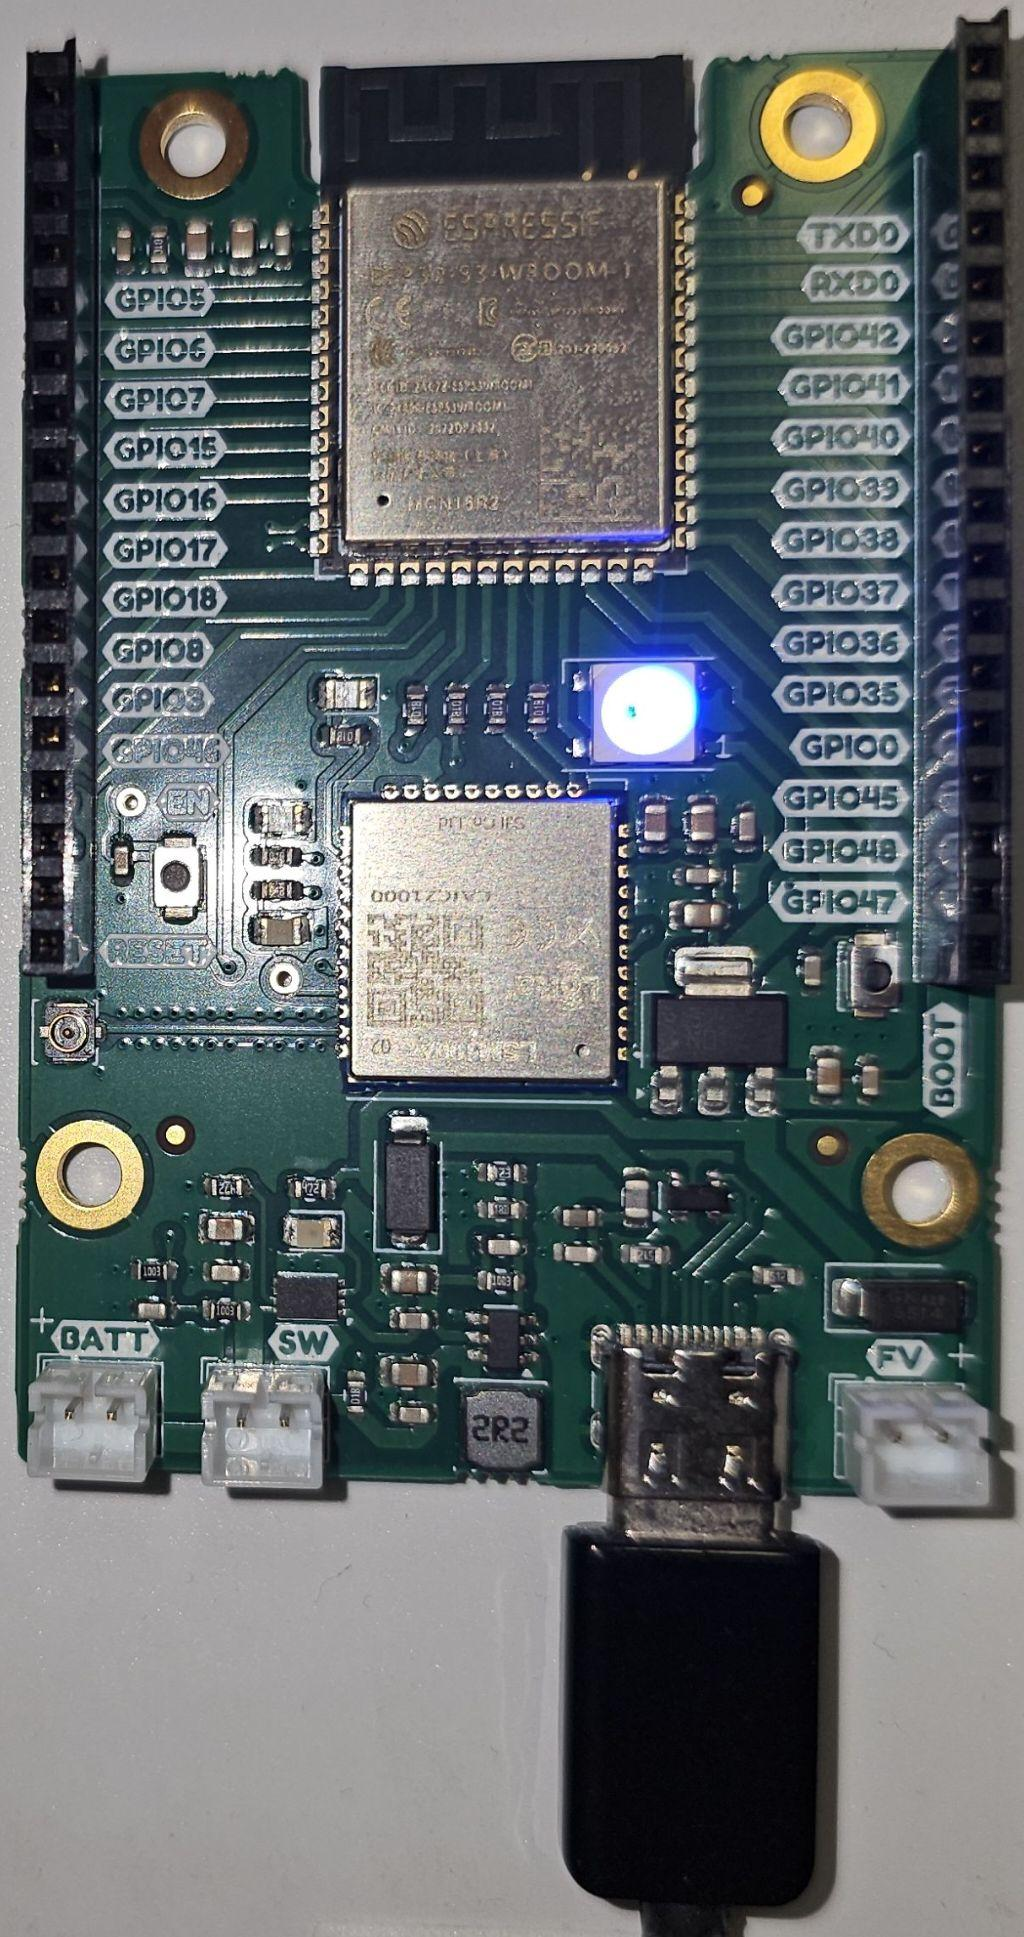
\includegraphics[width=4cm,angle=90]{../../Images/Syde/TestRGB};
    
    \captionof{figure}{Output after the download of the sketch \FILE{TestRGB.ino}}\label{fig:ArduinoBoardHypatiaConnectingState}
\end{center}	
        
        

\section{Troubleshooting}


\begin{enumerate}
  \item If you try to upload a new sketch to Hypatia and you get this error message ``A fatal error occurred: Failed to connect to ESP32: Timed out\ldots Connecting\ldots''. It means that your ESP32 is not in flashing/uploading mode.

  \bigskip
  
  Having the right board name and COM port selected, follow these steps:
  
  \begin{itemize}
    \item Hold-down the button ``Boot'' in your board
    \item Press the button ``Upload'' in the Arduino IDE to upload your sketch
    \item After you see the  message ``Connecting\ldots'' in your Arduino IDE, release the finger from the button ``Boot''
    \item After that, you should see the message ``Done uploading''
  \end{itemize}


  \medskip
  
  You'll also have to repeat that button sequence every time you want to upload a new sketch. But if you want to solve this issue once for all without the need to press the button ``Boot'', follow the suggestions in the next guide:

  \begin{itemize}
    \item \HREF{https://randomnerdtutorials.com/solved-failed-to-connect-to-esp32-timed-out-waiting-for-packet-header/}{[SOLVED] Failed to connect to ESP32: Timed out waiting for packet header}
  \end{itemize}

  \item  If you get the error ``COM Port not found/not available'', you might need to check the port: 

    \begin{itemize}
      \item Open Window's device manager using  \menu{Windows + X}.
      \item Check the usb ports.
     \end{itemize}

  \item  If you get the error ``COM Port not found/not available'', you might need to install the CP210x Drivers:

  \begin{itemize}
    \item \HREF{https://randomnerdtutorials.com/install-esp32-esp8266-usb-drivers-cp210x-windows/}{Install USB Drivers – CP210x USB to UART Bridge (Windows PC)}
    \item \HREF{https://randomnerdtutorials.com/install-esp32-esp8266-usb-drivers-cp210x-mac-os/}{Install USB Drivers – CP210x USB to UART Bridge (Mac OS X)}
  \end{itemize}

\end{enumerate}


If you experience any problems or issues with your board, take a look at our in-depth \HREF{https://randomnerdtutorials.com/esp32-troubleshooting-guide/}{ESP32 Troubleshooting Guide}.

